\documentclass[slideopt,A4,showboxes,svgnames]{beamer}

%% list of packages here
\usepackage[absolute,showboxes,overlay]{textpos}
\usepackage{mathtools}
\usepackage{amsmath}
\usepackage{amssymb}
\usepackage{pifont}
\usepackage{multicol}
\usepackage[linesnumbered,ruled,vlined]{algorithm2e}

\usepackage{theme/beamerthemeinria}



%%%%%%%%%%%%%%%%%%%%%%%%%%%%
% Paper dependent stuff    %
%%%%%%%%%%%%%%%%%%%%%%%%%%%%

\newcommand{\FTQ}{\textcolor{myalgocolor}{\normalfont \texttt{FTQ}}\xspace}
\newcommand{\FTQl}{\textcolor{myalgocolor}{\normalfont \texttt{FTQ}$(\lambda)$}\xspace}
\newcommand{\BFTQ}{\textcolor{myalgocolor}{\normalfont \texttt{BFTQ}}\xspace}
\newcommand{\ov}{\overline}
\newcommand{\oa}{\ov{a}}
\newcommand{\ox}{\ov{x}}
\newcommand{\oz}{\ov{z}}
\newcommand{\oy}{\ov{y}}
\newcommand{\os}{\ov{s}}
\newcommand{\ocS}{\ov{\cS}}
\newcommand{\ocA}{\ov{\cA}}

%%%%%%%%%%%%%%%%%%%%%%%%%%%%
% Aesthetics               %
% over-underline, hat, bold%
%%%%%%%%%%%%%%%%%%%%%%%%%%%%

\newcommand{\eps}{\varepsilon}
\newcommand{\vareps}{\varepsilon}
\renewcommand{\epsilon}{\varepsilon}
%\renewcommand{\hat}{\widehat}
\renewcommand{\tilde}{\widetilde}
\renewcommand{\bar}{\overline}

\newcommand*{\MyDef}{\mathrm{\tiny def}}
\newcommand*{\eqdefU}{\ensuremath{\mathop{\overset{\MyDef}{=}}}}% Unscaled version
\newcommand*{\eqdef}{\mathop{\overset{\MyDef}{\resizebox{\widthof{\eqdefU}}{\heightof{=}}{=}}}}


\def\:#1{\protect \ifmmode {\mathbf{#1}} \else {\textbf{#1}} \fi}
\newcommand{\CommaBin}{\mathbin{\raisebox{0.5ex}{,}}}

\newcommand{\wt}[1]{\widetilde{#1}}
\newcommand{\wh}[1]{\widehat{#1}}
\newcommand{\wo}[1]{\overline{#1}}
\newcommand{\wb}[1]{\overline{#1}}

% bf and bm missing due to conflict!!
\newcommand{\bsym}[1]{\mathbf{#1}}
\newcommand{\bzero}{\mathbf{0}}
\newcommand{\ba}{\mathbf{a}}
\newcommand{\bb}{\mathbf{b}}
\newcommand{\bc}{\mathbf{c}}
\newcommand{\bd}{\mathbf{d}}
\newcommand{\be}{\mathbf{e}}
\newcommand{\bbE}{\mathbb{E}}
\newcommand{\bg}{\mathbf{g}}
\newcommand{\bh}{\mathbf{h}}
\newcommand{\bi}{\mathbf{i}}
\newcommand{\bj}{\mathbf{j}}
\newcommand{\bk}{\mathbf{k}}
\newcommand{\bl}{\mathbf{l}}
\newcommand{\bn}{\mathbf{n}}
\newcommand{\bo}{\mathbf{o}}
\newcommand{\bp}{\mathbf{p}}
\newcommand{\bq}{\mathbf{q}}
\newcommand{\br}{\mathbf{r}}
\newcommand{\bs}{\mathbf{s}}
\newcommand{\bt}{\mathbf{t}}
\newcommand{\bu}{\mathbf{u}}
\newcommand{\bv}{\mathbf{v}}
\newcommand{\bw}{\mathbf{w}}
\newcommand{\bx}{\mathbf{x}}
\newcommand{\by}{\mathbf{y}}
\newcommand{\bz}{\mathbf{z}}

\newcommand{\bA}{\mathbf{A}}
\newcommand{\bB}{\mathbf{B}}
\newcommand{\bC}{\mathbf{C}}
\newcommand{\bD}{\mathbf{D}}
\newcommand{\bE}{\mathbf{E}}
\newcommand{\bF}{\mathbf{F}}
\newcommand{\bG}{\mathbf{G}}
\newcommand{\bH}{\mathbf{H}}
\newcommand{\bI}{\mathbf{I}}
\newcommand{\bJ}{\mathbf{J}}
\newcommand{\bK}{\mathbf{K}}
\newcommand{\bL}{\mathbf{L}}
\newcommand{\bM}{\mathbf{M}}
\newcommand{\bN}{\mathbf{N}}
\newcommand{\bO}{\mathbf{O}}
\newcommand{\bP}{\mathbf{P}}
\newcommand{\bQ}{\mathbf{Q}}
\newcommand{\bR}{\mathbf{R}}
\newcommand{\bS}{\mathbf{S}}
\newcommand{\bT}{\mathbf{T}}
\newcommand{\bU}{\mathbf{U}}
\newcommand{\bV}{\mathbf{V}}
\newcommand{\bW}{\mathbf{W}}
\newcommand{\bX}{\mathbf{X}}
\newcommand{\bY}{\mathbf{Y}}
\newcommand{\bZ}{\mathbf{Z}}

% calligraphic
\newcommand{\cf}{\mathcal{f}}
\newcommand{\cA}{\mathcal{A}}
\newcommand{\cB}{\mathcal{B}}
\newcommand{\cC}{\mathcal{C}}
\newcommand{\cD}{\mathcal{D}}
\newcommand{\cE}{\mathcal{E}}
\newcommand{\cF}{\mathcal{F}}
\newcommand{\cG}{\mathcal{G}}
\newcommand{\cH}{\mathcal{H}}
\newcommand{\cI}{\mathcal{I}}
\newcommand{\cJ}{\mathcal{J}}
\newcommand{\cK}{\mathcal{K}}
\newcommand{\cL}{\mathcal{L}}
\newcommand{\cM}{\mathcal{M}}
\newcommand{\cN}{\mathcal{N}}
\newcommand{\cO}{\mathcal{O}}
\newcommand{\cP}{\mathcal{P}}
\newcommand{\cQ}{\mathcal{Q}}
\newcommand{\cR}{\mathcal{R}}
\newcommand{\cS}{\mathcal{S}}
\newcommand{\cT}{\mathcal{T}}
\newcommand{\cU}{\mathcal{U}}
\newcommand{\cV}{\mathcal{V}}
\newcommand{\cW}{\mathcal{W}}
\newcommand{\cX}{\mathcal{X}}
\newcommand{\cY}{\mathcal{Y}}
\newcommand{\cZ}{\mathcal{Z}}

%%%%%%%%%%%%%%%%%%%%%%%%%%%%
% Math jargon              %
%%%%%%%%%%%%%%%%%%%%%%%%%%%%
\newcommand{\wrt}{w.r.t.\xspace}
\newcommand{\defeq}{\stackrel{\mathclap{\normalfont\mbox{\tiny def}}}{=}}
\newcommand{\maxund}[1]{\max\limits_{#1}}
\newcommand{\supund}[1]{\text{sup}\limits_{#1}}
\newcommand{\minund}[1]{\min\limits_{#1}}
\renewcommand{\epsilon}{\varepsilon}
\newcommand{\bigotime}{\mathcal{O}}


\DeclareMathOperator*{\argmin}{arg\,min}
\DeclareMathOperator*{\argmax}{arg\,max}
\DeclareMathOperator*{\cupdot}{\mathbin{\mathaccent\cdot\cup}}

%%%%%%%%%%%%%%%%%%%%%%%%%%%%
% Matrix operators         %
%%%%%%%%%%%%%%%%%%%%%%%%%%%%
\newcommand{\transpose}{^\mathsf{\scriptscriptstyle T}}
\newcommand{\transp}{\mathsf{\scriptscriptstyle T}}

%%%%%%%%%%%%%%%%%%%%%%%%%%%%
% Statistic operators      %
%%%%%%%%%%%%%%%%%%%%%%%%%%%%
\newcommand{\probability}[1]{\mathbb{P}\left(#1\right)}
\newcommand{\probdist}{Pr}
\DeclareMathOperator*{\expectedvalue}{\mathbb{E}}
\DeclareMathOperator*{\variance}{\text{Var}}
\newcommand{\expectedvalueover}[1]{\expectedvalue\limits_{#1}}
\newcommand{\condbar}{\;\middle|\;}
\newcommand{\gaussdistr}{\mathcal{N}}
\newcommand{\uniformdistr}{\mathcal{U}}
\newcommand{\bernoullidist}{\mathcal{B}}

%%%%%%%%%%%%%%%%%%%%%%%%%%%%
% Algebraic Sets           %
%%%%%%%%%%%%%%%%%%%%%%%%%%%%
\newcommand{\Real}{\mathbb{R}}
\newcommand{\Natural}{\mathbb{N}}
\newcommand{\statespace}{\mathcal{X}}
\newcommand{\funcspace}{\mathcal{F}}
\newcommand{\dynaspace}{\mathcal{T}}

%
%\newtheorem{theorem}{Theorem}
%\newtheorem{definition}{Definition}
%\newtheorem{lemma}{Lemma}
\newtheorem{proposition}{Proposition}
\newtheorem{remark}{Remark}
\newtheorem{conjecture}{Conjecture}
%\newtheorem{property}{Property}
%\newtheorem{assumption}{Assumption}
%\newtheorem{conjecture}{Conjecture}
%
%\newtheorem*{definition*}{Definition}
%\newtheorem*{theorem*}{Theorem}
%\newtheorem*{proposition*}{Proposition}
%\newtheorem*{remark*}{Remark}



% Arrows
\newcommand{\incarrow}{{
\includegraphics[height=0.7\baselineskip]{./img/arrow_list}}}
\newcommand{\xmark}{\ding{55}}%


% Colors for slides
\definecolor{rouge1}{RGB}{226,0,38}  % red P
\definecolor{orange1}{RGB}{243,154,38}  % orange P
\definecolor{jaune}{RGB}{254,205,27}  % jaune P
\definecolor{blanc}{RGB}{255,255,255} % blanc P

\definecolor{rouge2}{RGB}{230,68,57}  % red S
\definecolor{orange2}{RGB}{236,117,40}  % orange S
\definecolor{taupe}{RGB}{134,113,127} % taupe S
\definecolor{gris}{RGB}{91,94,111} % gris S
\definecolor{bleu1}{RGB}{38,109,131} % bleu S
\definecolor{bleu2}{RGB}{28,50,114} % bleu S
\definecolor{vert1}{RGB}{133,146,66} % vert S
\definecolor{vert3}{RGB}{20,200,66} % vert S
\definecolor{vert2}{RGB}{157,193,7} % vert S
\definecolor{vertsolarized}{RGB}{211,233,219} % vert S
\definecolor{darkyellow}{RGB}{233,165,0}  % orange S
\definecolor{lightgray}{rgb}{0.9,0.9,0.9}
\definecolor{darkgray}{rgb}{0.6,0.6,0.6}

% Highlights for slides
\newcommand{\rcol}[1]{\textcolor{red}{\textit{#1}}}
%\newcommand{\eqrcol}[1]{\textcolor{red}{#1}}
%\newcommand{\eqrcolb}[1]{\textcolor{red}{\boldsymbol{#1}}}
\newcommand{\gcol}[1]{\textcolor{vert3}{\textit{#1}}}
%\newcommand{\eqgcol}[1]{\textcolor{vert3}{#1}}
%\newcommand{\eqgcolb}[1]{\textcolor{vert3}{\boldsymbol{#1}}}
\newcommand{\blcol}[1]{\textcolor{blue}{\textit{#1}}}
%\newcommand{\eqbcol}[1]{\textcolor{blue}{#1}}
%\newcommand{\eqbcolb}[1]{\textcolor{blue}{\boldsymbol{#1}}}
\newcommand{\ycol}[1]{\textcolor{darkyellow}{\textit{#1}}}
\newcommand{\eqycol}[1]{\textcolor{darkyellow}{#1}}

\newcommand{\rcolbm}[1]{$\textcolor{red}{\boldsymbol{#1}}$}
\newcommand{\rcolb}[1]{\textcolor{red}{\textit{\textbf{#1}}}}
\newcommand{\gcolb}[1]{\textcolor{vert3}{\textit{\textbf{#1}}}}
\newcommand{\bcolb}[1]{\textcolor{blue}{\textit{\textbf{#1}}}}
\newcommand{\ycolb}[1]{\textcolor{darkyellow}{\textit{\textbf{#1}}}}

% Colored boxes
\newcounter{ColoredBoxesCounter}
\newcommand{\highlightnew}[3][(0.0,-0.1)(-0.0,0.3)]{
\hfsetfillcolor{#2!20}
\hfsetbordercolor{#2!80}
\tikzmarkin{\theColoredBoxesCounter}#1
#3
\tikzmarkend{\theColoredBoxesCounter}
\stepcounter{ColoredBoxesCounter}
}

\newcommand{\highlight}[2][yellow]{\mathchoice%
{\colorbox{#1}{$\displaystyle#2$}}%
{\colorbox{#1}{$\textstyle#2$}}%
{\colorbox{#1}{$\scriptstyle#2$}}%
{\colorbox{#1}{$\scriptscriptstyle#2$}}}%

\newcommand{\eqrcol}[1]{\highlight[red!20]{#1}}
\newcommand{\eqrcolb}[1]{\highlight[red!20]{\boldsymbol{#1}}}
\newcommand{\eqgcol}[1]{\highlight[vert3!20]{#1}}
\newcommand{\eqgcolb}[1]{\highlight[vert3!20]{\boldsymbol{#1}}}
\newcommand{\eqbcol}[1]{\highlight[blue!20]{#1}}
\newcommand{\eqbcolb}[1]{\highlight[blue!20]{\boldsymbol{#1}}}

\colorlet{redp}{red!20} % vert S
\colorlet{greenp}{vert3!20} % vert S
\colorlet{bluep}{blue!20} % vert S
\colorlet{yellowp}{yellow!20} % vert S

\newcommand{\hl}[3][\fboxsep1pt]{{#1\colorbox{#2}{#3}}}%

\newcommand{\hlr}[1]{\hl{redp}{#1}}
\newcommand{\hlg}[1]{\hl{greenp}{#1}}
\newcommand{\hlb}[1]{\hl{bluep}{#1}}
\newcommand{\hly}[1]{\hl{yellowp}{#1}}

\newcommand{\hler}[1]{\hl[\fboxsep0pt]{redp}{$\displaystyle {#1}$}}
\newcommand{\hleg}[1]{\hl[\fboxsep0pt]{greenp}{$\displaystyle {#1}$}}
\newcommand{\hleb}[1]{\hl[\fboxsep0pt]{bluep}{$\displaystyle {#1}$}}

\newcommand{\hlbr}[1]{\hl[\fboxsep0pt]{redp}{$\displaystyle \mathbf{#1}$}}
\newcommand{\hlbg}[1]{\hl[\fboxsep0pt]{greenp}{$\displaystyle \mathbf{#1}$}}
\newcommand{\hlbb}[1]{\hl[\fboxsep0pt]{bluep}{$\displaystyle \mathbf{#1}$}}

\newcommand{\vph}{\vphantom{A_A^A}}

% Box for algorithms
\newlength{\minipagewidth}
\newlength{\minipagewidthx}
\setlength{\minipagewidth}{\columnwidth}
\setlength{\minipagewidthx}{\columnwidth}
\setlength{\fboxsep}{0.1mm}
\addtolength{\minipagewidth}{-\fboxrule}
\addtolength{\minipagewidth}{-\fboxrule}
\addtolength{\minipagewidth}{-\fboxsep}
\addtolength{\minipagewidth}{-\fboxsep}
\addtolength{\minipagewidthx}{+\fboxsep}
\newcommand{\bookbox}[1]{\small
\par\medskip\noindent
\framebox[\columnwidth]{
\begin{minipage}{\minipagewidth} {#1} \end{minipage} } \par\medskip }

\newcommand{\bookboxx}[1]{
\par\medskip\noindent
\framebox[\columnwidth]{
\begin{minipage}[t]{0.98\columnwidth} {\par\smallskip#1\par\smallskip} \end{minipage} } \par\medskip }


\usepackage{array}
\newcolumntype{L}[1]{>{\raggedright\let\newline\\\arraybackslash\hspace{-3.1cm}}m{#1}}
\newcolumntype{C}[1]{>{\centering\let\newline\\\arraybackslash\hspace{135pt}}m{#1}}
\newcolumntype{R}[1]{>{\raggedleft\let\newline\\\arraybackslash\hspace{-10pt}}m{#1}}

\newenvironment{myfont}{\fontfamily{kurier}\selectfont}{\par}
\newenvironment{myfont2}{\fontfamily{epigrafica}\selectfont}{\par}

% Border color of content boxes
\definecolor{bordercol}{RGB}{0,0,0}  %black
% Background color for the header in the content boxes (left side)
\definecolor{headercol1}{RGB}{200,0,0}        %red:RGB {200,0,0} 
% Background color for the header in the content boxes (right side) 
\definecolor{headercol2}{rgb}{1.0,0.49,0.0}        %orange:rgb {1.0,0.49,0.0}
% Text color for the header text in the content boxes
\definecolor{headerfontcol}{rgb}{1,1,1}  %white
% Background color for the content in the boxes
\definecolor{boxcolor}{rgb}{1,1,1} 

\definecolor{lightblue}{rgb}{0.145,0.6666,1}

\newsavebox\CBox
\newcommand\hcancel[2][0.5pt]{%
  \ifmmode\sbox\CBox{$#2$}\else\sbox\CBox{#2}\fi%
  \makebox[0pt][l]{\usebox\CBox}%  
  \rule[0.3\ht\CBox-#1/2]{\wd\CBox}{#1}}


\title[Budgeted Reinforcement Learning]{Budgeted Reinforcement Learning\\in Continuous State Space}
\subtitle{Sous-titre}
\date[date]{date}
\author[Carrara et al.]{Nicolas Carrara\inst{1},
	Edouard Leurent\inst{1,2},\\
	Tanguy Urvoy\inst{3},
	Romain Laroche\inst{4},\\
	Odalric Maillard\inst{1},
	Olivier Pietquin\inst{1,5}}
\institute{
	\inst{1} Inria SequeL, 
	\inst{2} Renault Group,\\
	\inst{3} Orange Labs,
	\inst{4} Microsoft Montr\'eal,\\
	\inst{5} Google Research, Brain Team}

\begin{document}

\begin{frame}
    \titlepage
\end{frame}


\frame{\tocpage}
 
\section{Setting}
\frame{\sectionpage}


\begin{frame}{Motivation}

\begin{alertblock}{Conflicting Objectives}
Single scalar reward to represent multiple contradictory aspects (task completion vs safety)

No explicit control over the tradeoffs
\end{alertblock}

Examples?


\end{frame}

\begin{frame}{Constrained Reinforcement Learning}
\begin{block}{\only<2>{Constrained} Markov Decision Process}
	A\only<1>{n} \alert<2>{\only<2>{C}MDP} is a tuple $(\cS, \cA, P, \Rr, \only<2>{\alert<2>{R_c,}} \gamma \only<2>{\alert{, \beta}})$ with:
	\begin{multicols}{2}
			\begin{itemize}
			\item Rewards $\Rr\in\Real^{\cS \times \cA}$
			\item[]
			\item<2> \alert<2>{Costs $R_c\in\Real^{\cS \times \cA}$}
			\item<2> \alert{Budget $\beta$}
		\end{itemize}
	\end{multicols}
\end{block}
\begin{block}{Objective}
Find $\pi^*$ such that $\forall s\in\cS$:
	\begin{equation*}
	\begin{array}{lcr}
	\displaystyle \pi^* \in \argmax_{\pi\in\cM(\cA)^{\cS}} \expectedvalue\left[\sum_{t=0}^\infty \gamma^t \Rr(s_t, a_t) \condbar s_0=s \right]\\
	\visible<2>{
	\text{ s.t. }  \displaystyle \alert<2>{\expectedvalue\left[\sum_{t=0}^\infty \gamma^t R_c(s_t, a_t) \condbar s_0=s\right] \leq \beta}}
	\end{array}
	\end{equation*}
\end{block}
\end{frame}

\begin{frame}{Budgeted Reinforcement Learning}
\begin{block}{Budgeted Markov Decision Process}
	A \alert{BMDP} is a tuple $(\cS, \cA, P, \Rr, \Rc, \gamma\alert{, \cB})$ with:
	\begin{multicols}{2}
		\begin{itemize}
			\item Rewards $\Rr\in\Real^{\cS \times \cA}$
			\item[]
			\item Costs $\Rc\in\Real^{\cS \times \cA}$
			\item \alert{Budget space $\cB$}
		\end{itemize}
	\end{multicols}
\end{block}
\begin{block}{Objective}
	Find $\pi^*$ such that $\forall\alert{(s,\beta)\in\cS\times\cB}$:
	\begin{equation*}
	\begin{array}{lcr}
	\displaystyle \pi^* \in \argmax_{\pi\in\cM(\cA \alert{\times \cB})^{\cS\alert{\times \cB}}} \expectedvalue\left[\sum_{t=0}^\infty \gamma^t R_r(s_t, a_t) \condbar s_0=s, \alert{\beta_0 = \beta}\right]\\
		\text{ s.t. }  \displaystyle \expectedvalue\left[\sum_{t=0}^\infty \gamma^t \Rc(s_t, a_t) \condbar s_0=s, \alert{\beta_0 = \beta}\right] \leq \beta
	\end{array}
	\end{equation*}
\end{block}
\end{frame}

\begin{frame}{Augmented Settings}
Budgeted policies $\pi$
\begin{itemize}
	\item Take a budget $\beta$ as an additional input
	\item Output a next budget $\beta'$ 
	\item $\pi:\underbrace{(s,\beta)}_{\os} \rightarrow \underbrace{(a,\beta')}_{\oa}$
\end{itemize}

\end{frame}


\begin{frame}{Augmented Setting}

\begin{alertblock}{Definition (Augmented spaces)}
	\begin{itemize}
		\item States $\ocS = \cS\times\cB$.
		\item Actions $\ocA = \cA\times\cB$.
		\item Dynamics $\ov{P}$
		\vspace*{-0.5cm}
		\[\text{state } (s,\beta), \text{ action }(a, \beta_a) \rightarrow \text{ next state }\begin{cases}s'\sim P(s'|s, a)\\\beta' = \beta_a\end{cases}\]
	\end{itemize}
\end{alertblock}

\begin{alertblock}{Definition (Augmented signals)}
	\begin{enumerate}
		\item Rewards $R = ({\green R_r}, {\red R_c})$
		\item Returns $G^\pi = ({\green G_r^\pi}, {\red G_c^\pi}) \eqdef \sum_{t=0}^\infty \gamma^t R(\os_t,\oa_t)$
		\item Value $V^\pi(\os) = ({\green V_r^\pi}, {\red V_c^\pi}) \eqdef \expectedvalue\left[ G^\pi \condbar \ov{s_0} = \os\right]$
		\item Q-Value $Q^\pi(\os, \oa)= ({\green Q_r^\pi}, {\red Q_c^\pi}) \eqdef \expectedvalue\left[ G^\pi \condbar \ov{s_0} = \os, \ov{a_0} = \oa\right]$
	\end{enumerate}
\end{alertblock}
\end{frame}

\section{Budgeted Dynamic Programming}
\frame{\sectionpage}


\begin{frame}{Policy Evaluation}
\begin{proposition}[Budgeted Bellman Expectation]
	The Bellman Expectation equations are \alert{preserved}
	\begin{align*}
	V^\pi(\os) = \sum_{\oa\in\ocA}\pi(\oa | \os) Q^\pi(\os, \oa) \\ Q^\pi(\os, \oa) = R(\os, \oa) + \gamma\sum_{\os'\in\ocS}\ov{P}\left(\os' \condbar \os, \oa\right) V^\pi(\os') 
	\end{align*}
\end{proposition}
\pause
\begin{proposition}[Contraction]
	The Bellman Expectation Operator $\cT^\pi$ is a $\gamma$-contraction.
	\begin{align*}
	\cT^\pi Q(\os, \oa) &\eqdef R(\os, \oa) + \gamma \sum_{\os'\in\ocS}\sum_{\oa'\in\ocA}\ov{P}(\os'|\os, \oa)\pi(\oa'|\os') Q(\os', \oa')
	\end{align*}
\end{proposition}

\begin{itemize}
	\item[\green \checkmark] We can {\green evaluate} a budgeted policy $\pi$
\end{itemize}
\end{frame}

\begin{frame}{Budgeted Optimality}
\begin{alertblock}{Definition (Budgeted Optimality)}
	In that order, we want to:
	\begin{enumerate}
		\item[(i)] {\red Respect the budget $\beta$}: 
		\begin{equation*}
		\Pi_a(\os) \eqdef \{\pi\in\Pi: V_c^\pi(s, \beta) \hler{\leq \beta}\}
		\end{equation*}
		\item[(ii)] {\green Maximise the rewards}:
		\begin{equation*}
		V_r^*(\os) \eqdef \hleg{\max}_{\pi\in\Pi_a(\os)}  V_r^\pi(\os) \quad\quad \Pi_r(\os) \eqdef \hleg{\argmax}_{\pi\in\Pi_a(\os)}  V_r^\pi(\os)
		\end{equation*}
		\item[(iii)] \alert{Minimise the costs}: 
		\begin{equation*}
		V_c^*(\os) \eqdef \hleb{\min}_{\pi\in\Pi_r(\os)}  V_c^\pi(\os), \quad\quad \Pi^*(\os) \eqdef \hleb{\argmin}_{\pi\in\Pi_r(\os)}  V_c^\pi(\os)
		\end{equation*}
	\end{enumerate}
\end{alertblock}
We define the budgeted action-value function $Q^*$ similarly
\end{frame}

\begin{frame}{Budgeted Optimality}
\begin{theorem}[Budgeted Bellman Optimality Equation]
	$Q^*$ verifies the following equation:
	\begin{align*}
	Q^{*}(\os, \oa) &= \cT Q^{*}(\os, \oa)\\
	&\eqdef R(\os, \oa) + \gamma \sum_{\os'\in\ocS} \ov{P}(\ov{s'} | \os, \oa)\sum_{\ov{a'}\in \ocA} \pi_\text{greedy}(\ov{a'}|\ov{s'}; Q^*) Q^{*}(\ov{s'}, \ov{a'})
	\end{align*}
\end{theorem}
where the greedy policy {$\pi_\text{greedy}$} is defined by:
\begin{align*}
\pi_\text{greedy}(\oa|\os; Q) \in &\hleb{\argmin}_{\rho\in\Pi_r^Q} \expectedvalueover{\oa\sim\rho}Q_c(\os, \oa), \\
\text{where }\quad \Pi_r^Q \eqdef &\hleg{\argmax}_{\rho\in\cM(\ocA)} \expectedvalueover{\oa\sim\rho} Q_r(\os, \oa) \\
& \text{ s.t. }  \expectedvalueover{\oa\sim\rho} Q_c(\os, \oa) \hler{\leq \beta}
\end{align*}
\end{frame}

\begin{frame}{The optimal policy}
\begin{proposition}[Optimality of the policy]
	$\pi_\text{greedy}(\cdot~; Q^*)$ is \alert{simultaneously optimal} in all states $\os\in\ocS$: $$\pi_\text{greedy}(\cdot~; Q^*)\in \alert{\Pi^*(\os)}$$
	
	In particular, $V^{\pi_\text{greedy}(\cdot; Q^*)} = V^*$ and $Q^{\pi_\text{greedy}(\cdot; Q^*)}= Q^*$.
\end{proposition}

\begin{proposition}[Solving the non-linear program]
	$\pi_\text{greedy}$ can be computed \alert{efficiently}, as a mixture $\pi_\text{hull}$ of two points that lie on the convex hull of $Q$.
	\[\pi_{\text{greedy}}=\pi_\text{hull}\]
\end{proposition}
\end{frame}

\foreach \n in {0,1,2,3,4}{
	\begin{frame}{Solving the non-linear program: intuition}
	\begin{figure}
		\centering
		\includegraphics[scale=1.0,page=1]{img/b\n}
	\end{figure}
\end{frame}
}

\begin{frame}{Convergence analysis}
Recall what we've shown so far:
\[\cT \xrightarrow[fixed-point]{} Q^* \xrightarrow[tractable]{} \pi_{\text{hull}}(Q^*) \xrightarrow[equal]{} \pi_{\text{greedy}}(Q^*) \xrightarrow[optimal]{} \]

\pause
We're {\green almost there}! 

All that is left is to perform \alert{Fixed-Point Iteration} to compute $Q^*$.

\pause
\begin{theorem}[Non-Contractivity]
For any BMDP ($\cS,\cA,P,R_r,R_c,\gamma$) with $|\cA| \geq 2$, $\cT$ is \textbf{\red not} a contraction.
$$\forall\epsilon>0, \exists Q^1,Q^2\in(\Real^2)^{\ocS\ocA}:\|\cT Q^1-\cT Q^2\|_\infty \geq \frac{1}{\epsilon}\|Q^1-Q^2\|_\infty$$
\end{theorem}

\begin{itemize}
	\item[\red \xmark] We {\red cannot guarantee} the convergence of $\cT^n(Q_0)$ to $Q^*$
\end{itemize}
\end{frame}

\foreach \n in {0,1,2}{
	\begin{frame}{Not a contraction: intuition}
	\begin{figure}
		\centering
		\includegraphics[scale=0.9,page=1]{img/d\n}
	\end{figure}
	\end{frame}
}

\begin{frame}{Convergence analysis}
Thankfully,
\begin{theorem}[Contractivity on smooth Q-functions]
	$\cT$ \alert{is a contraction} when restricted to the subset $\cL_\gamma$ of $Q$-functions such that "$Q_r$ is $L$-Lipschitz with respect to $Q_c$", with $L<\frac{1}{\gamma}-1$.
\end{theorem}
\begin{equation*}
\cL_\gamma = \left\{\begin{array}{cc}
Q\in(\Real^2)^{\ocS\ocA}\text{ s.t. }\exists L<\frac{1}{\gamma}-1: \forall \os\in\ocS,\oa_1,\oa_2\in\ocA,   \\
|Q_r(\os,\oa_1) - Q_r(\os,\oa_2)| \leq L|Q_c(\os,\oa_1) - Q_c(\os,\oa_2)|
\end{array}\right\}
\end{equation*}
\begin{itemize}
	\item[\green \checkmark] We {\green guarantee} convergence under some (strong) assumptions
	\item[\green \checkmark] We {\green observe} empirical convergence
\end{itemize}
\end{frame}

\begin{frame}{Budgeted Dynamic Programming}
\begin{center}
	\scalebox{0.9}{
		\begin{algorithm}[H]
			\DontPrintSemicolon
			\KwData{$P, R_r, R_c$}
			\KwResult{$Q^*$}
			$Q_{0} \leftarrow 0$\;
			\Repeat{convergence}{
				$Q_{k+1} \leftarrow \cT Q_k$\;
			}
			\caption{Budgeted Value-Iteration}
		\end{algorithm}
	}
\end{center}
\end{frame}

\section{Budgeted Reinforcement Learning}
\frame{\sectionpage}

\begin{frame}{Extension to the RL setting}

We address several limitations of Budgeted Value-Iteration

\begin{enumerate}[<+->]
	\item If the $P$, $R_r$ and $R_c$ are unknown:
	\begin{itemize}[<+->]
		\item Work with a {batch} of samples $\cD=\{(\os_i,\oa_i,r_i,\os_i'\}_{i\in [0,N]}$
		\item Replace $\cT$ with a sampling operator $\hat{\cT}$:
		\begin{equation*}
		\hat{\cT} Q(\os_i, \oa_i, r_i, \os'_i) \eqdef r_i + \gamma \sum_{\ov{a'_i}\in \cA_i} \pi_\text{greedy}(\ov{a'_i}|\ov{s'_i}; Q) Q(\ov{s'_i}, \ov{a'_i}).
		\end{equation*}
	\end{itemize}
	\item If $\cS$ is continuous:
	\begin{itemize}
		\item Employ function approximation $Q_\theta$, and minimise a regression loss
		$$\cL(Q_\theta, Q_\text{target};\cD) = \sum_{\cD} ||Q_\theta(\os, \oa) - Q_\text{target}(\os, \oa, r, \os')||_2^2$$
	\end{itemize}
	
\end{enumerate}

\end{frame}

\begin{frame}{More scaling}

\begin{itemize}[<+->]
\item CPU parallel computing of the targets $\sum_{\ov{a'_i}\in \cA_i} \pi_\text{greedy}(\ov{a'_i}|\ov{s'_i}; Q) Q(\ov{s'_i}, \ov{a'_i})$
\item Same for interactions with the environment.
\item Neural Network for function approximation: 
\begin{center}
	\resizebox{.5\textwidth}{!}{%
		
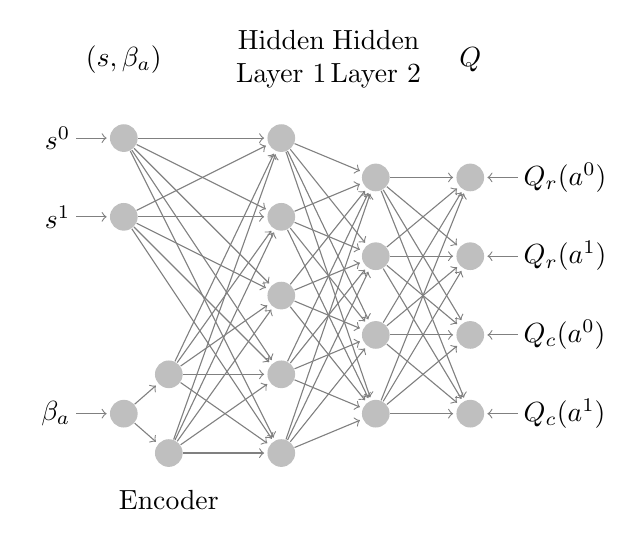
\begin{tikzpicture}[shorten >=1pt,->,draw=black!50, inner sep=1pt, node distance=\layersep]
        \tikzstyle{every pin edge}=[<-,shorten <=1pt]
        \tikzstyle{neuron}=[circle,fill=black!25,minimum size=10pt,inner sep=0pt]
        \tikzstyle{input neuron}=[neuron];
        \tikzstyle{input beta}=[neuron];
        \tikzstyle{qc}=[neuron];
        \tikzstyle{qr}=[neuron];
        \tikzstyle{hidden neuron}=[neuron];
        \tikzstyle{autoencoder neuron}=[neuron];
        \tikzstyle{annot} = [text width=4em, text centered]
        \tikzstyle{annot2} = [text width=10em, text centered]
        \def\layersep{2cm}
        % Draw the input layer nodes
        \foreach \name / \y in {0,...,1}
            \pgfmathtruncatemacro{\y}{0 + \y}
            \node[input neuron, pin=left:$s^\y$] (I-\name) at (0,-\y) {};

         % first layer
        \foreach \name / \y in {0,...,4}
        \pgfmathtruncatemacro{\y}{0 + \y}
            \path node[hidden neuron] (H1-\name) at (1*\layersep,-\y cm) {};

        \foreach \source in {0,...,1}
            \foreach \dest in {0,...,4}
                \path (I-\source) edge (H1-\dest);

        % BETA
        \node[input beta, pin=left:$\beta_a$] (BETA) at (0,-3.5) {};

        % beta auto encoder
        \foreach \name / \y in {0,...,1}
            \pgfmathtruncatemacro{\ybis}{3+ \y}
            \path node[autoencoder neuron] (AE-\name) at (\layersep/3.5,-\ybis cm) {};



        \foreach \name / \y in {0,...,3}
        \pgfmathtruncatemacro{\y}{0 + \y}
            \path[yshift=-0.5cm]
            node[hidden neuron] (H2-\name) at (1.6*\layersep,-\y cm) {};


        % actions
        \foreach \name / \y in {0,...,1}
        \pgfmathtruncatemacro{\y}{0 + \y}
            \path[yshift=-0.5cm] node[qr,pin=right:$Q_r(a^\y)$] (Qr-\name) at (2.2*\layersep,-\y cm) {};

        \foreach \name / \y in {0,...,1}
        \pgfmathtruncatemacro{\yy}{2 + \y}
            \path[yshift=-0.5cm] node[qc,pin=right:$Q_c(a^\y)$] (Qc-\name) at (2.2*\layersep,-\yy cm) {};

        \foreach \source in {0,...,1}
            \foreach \dest in {0,...,4}
                \path (AE-\source) edge (H1-\dest);



        \foreach \dest in {0,...,1}
            \path (BETA) edge (AE-\dest);

         \foreach \source in {0,...,4}
            \foreach \dest in {0,...,3}
                \path (H1-\source) edge (H2-\dest);

        \foreach \source in {0,...,3}
            \foreach \dest in {0,...,1}
                \path (H2-\source) edge (Qr-\dest);

         \foreach \source in {0,...,3}
            \foreach \dest in {0,...,1}
                \path (H2-\source) edge (Qc-\dest);
        % Annotate the layers
       \node[annot] (input) at (0,1) {$(s,\beta_a)$};
       \node[annot2] (input) at (\layersep/3.5,-4.6) {Encoder};
       \node[annot](h1) at (\layersep,1) {Hidden Layer 1};
       \node[annot](h2) at(1.6* \layersep,1) {Hidden Layer 2};
       \node[annot](output) at(2.2* \layersep,1) {$Q$};
        %\node[annot,right of=hl] {Output layer};
    \end{tikzpicture}

	}
\end{center}
\end{itemize}
\end{frame}

\section{Experiments}
\frame{\sectionpage}

\begin{frame}{Performances}
\begin{itemize}
	\item Baseline: $\lambda$-FTQ, Lagrangian relaxation
	\begin{itemize}
		\item $R_r(s,a) \leftarrow R_r(s,a) - \lambda R_c(s,a) \text{ where } \lambda \geq 0$
	\end{itemize}.
\end{itemize}
\end{frame}

\begin{frame}{Dialogue systems}
A slot-filling problem: the agent (the dialogue system) fills a form by asking the user each slot. It can either:
\begin{itemize}
	\item ask to answer using {\green voice} {\green (safe/slow)};
	\item ask to answer with a {\red numeric pad} {\red (unsafe/fast)}.
\end{itemize}


\begin{center}
	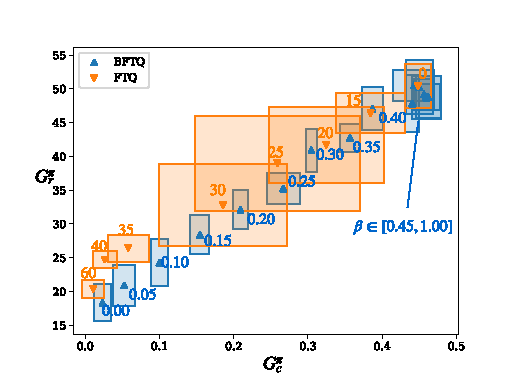
\includegraphics[trim={0 0.1cm 0 0.8cm}, clip, width=0.6\textwidth]{../../source/img/slot-filling.pdf}
\end{center}
\end{frame}


\begin{frame}{Autonomous driving}

The agent (the car) is on a two-way road with a car in front of it,
\begin{itemize}
	\item it can {\green stay behind} {\green (safe/slow)};
	\item it can {\red overtake} {\red (unsafe/fast)}.
	\end{itemize}

\begin{center}
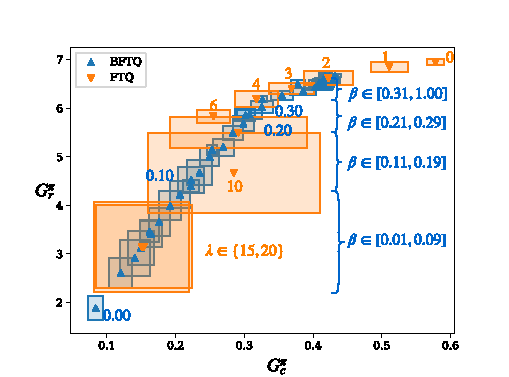
\includegraphics[trim={0 0cm 0 0.8cm}, clip, width=0.5\textwidth]{../../source/img/highway.pdf}\\
\href{https://budgeted-rl.github.io/\#driving-styles}{
\includegraphics[width=0.5\linewidth]{img/highway_env}}
\end{center}
			
\end{frame}

\begin{frame}{Risk-sensitive exploration}
\begin{alertblock}{How to collect the batch $\cD$?}
We propose an $\epsilon$-greedy exploration procedure:
\pause
\begin{itemize}[<+->]
	\item Sample an initial budget $\beta_0\sim\cU(\cB)$
	\item At each step, where $\os=(s,\beta)$ only explore feasible budgets:
	\begin{align*}
	&\oa = (a, \beta_a)\sim\mathcal{U}(\Delta_{\cA\cB})\\
	&\text{ where }  \Delta \text{ is such that }\probability{a, \beta_a|s, \beta} \text{verifies} \expectedvalue[\beta_a]\leq\beta
	\end{align*}
\end{itemize}
\end{alertblock}
\end{frame}

\begin{frame}{Corridors}

Two corridors:
\begin{enumerate}
\item one with {\red high costs / high rewards}
\item the other with {\green no costs / low rewards}
\end{enumerate}

\begin{center}
	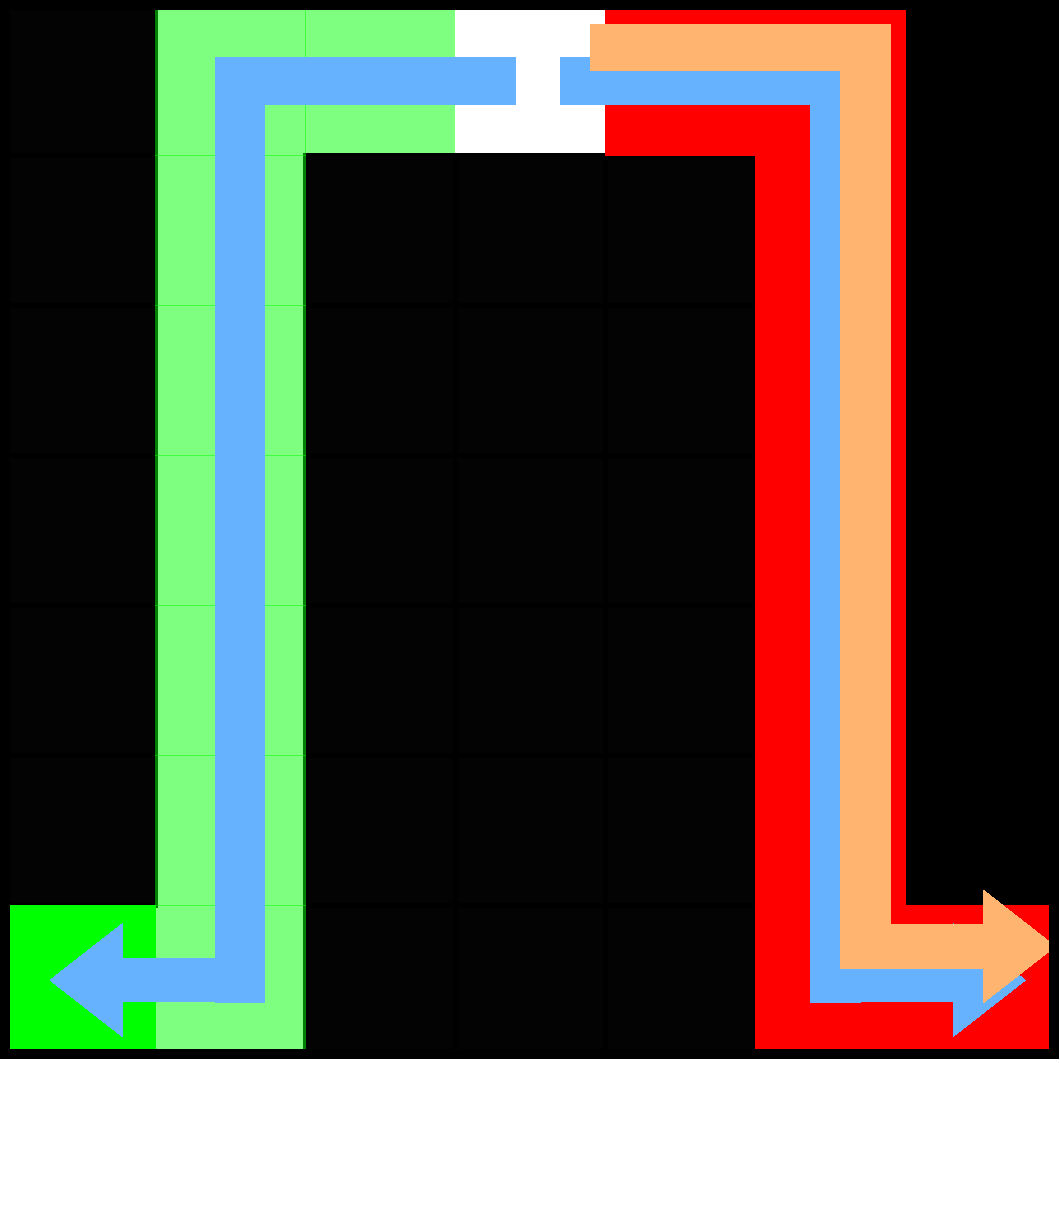
\includegraphics[width=0.3\textwidth]{../../source/img/corridors_paths}
\end{center}

\begin{itemize}
	\item[$\rightarrow$] Validate the \alert{risk-sensitive exploration} procedure
\end{itemize}

\end{frame}


\begin{frame}{Corridors}

\begin{columns}
\begin{column}{0.5\linewidth}
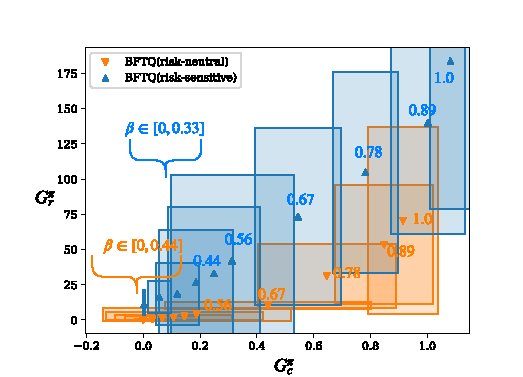
\includegraphics[trim={0.5cm 0.1cm 0.7cm 0.2cm}, clip, page=1, width=\linewidth]{../../source/img/corridors}
\end{column}
\begin{column}{0.46\linewidth}
\begin{center}
\href{https://budgeted-rl.github.io/\#risk-sensitive-exploration}{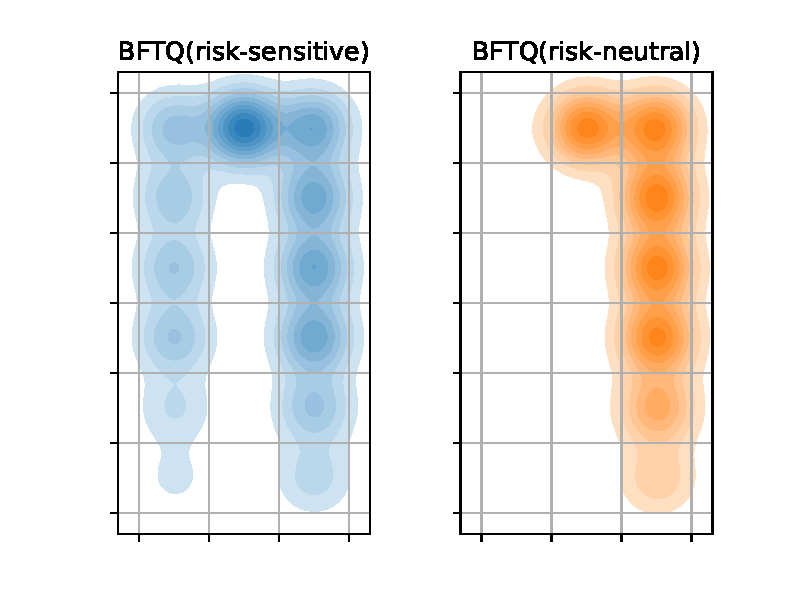
\includegraphics[trim={2cm 0.1cm 1cm 0.5cm}, clip, width=\linewidth]{../../source/img/corridors_densities.pdf}}
\end{center}
\end{column}
\end{columns}
\end{frame}


\end{document}
